\documentclass[11pt,class=report,crop=false]{standalone}
\usepackage[screen]{../python}

\begin{document}

%====================================================================
\chapitre{Principales fonctions}
%====================================================================


%%%%%%%%%%%%%%%%%%%%%%%%%%%%%%%%%%%%%%%%%%%%%%%%%%%%
\section{Mathématiques}

\textbf{Opérations classiques}
\begin{itemize}
  \item \ci{a + b},\quad \ci{a - b},\quad \ci{a * b}\quad  opérations classiques
  \item \ci{a / b}\quad division \og{}réelle\fg{} (renvoie un nombre flottant)
  \item \ci{a // b}\quad quotient de la division euclidienne (renvoie un entier)
  \item \ci{a \% b}\quad reste de la division euclidienne, appelé $a$ modulo $b$
  \item \ci{abs(x)}\quad valeur absolue
  \item \ci{x ** n}\quad puissance $x^n$
  \item \ci{4.56e12}\quad pour $4,56 \times 10^{12}$
\end{itemize}

\bigskip

\textbf{Module \og{}math\fg{}}

L'usage d'autres fonctions mathématiques nécessite le recours au module \ci{math} qui s'appelle par la commande :\\
\centerline{\ci{from math import *}}

\begin{itemize}
  \item \ci{sqrt(x)}\quad racine carrée $\sqrt{x}$
  \item \ci{cos(x)},\quad \ci{sin(x)},\quad \ci{tan(x)}\quad fonctions trigonométriques $\cos x$, $\sin x$, $\tan x$ en radians
  \item \ci{pi}\quad valeur approchée de $\pi = 3.14159265\ldots$
  \item \ci{floor(x)}\quad  entier juste en-dessous de $x$
  \item \ci{ceil(x)}\quad  entier juste au-dessus de $x$
  \item \ci{gcd(a,b)}\quad pgcd de $a$ et de $b$
 \end{itemize}
 \bigskip

\textbf{Module \og{}random\fg{}}

Le module \ci{random} génère des nombres de façon pseudo-aléatoire. Il s'appelle par la commande :\\
\centerline{\ci{from random import *}}

\begin{itemize}
  \item \ci{random()}\quad à chaque appel, renvoie un nombre flottant $x$ au hasard vérifiant  $0 \le x < 1$.
  \item \ci{randint(a,b)} \quad à chaque appel, renvoie un nombre entier $n$ au hasard vérifiant $a \le n \le b$.
  \item  \ci{choice(liste)} \quad à chaque appel, tire au hasard un élément de la liste.
  \item \ci{liste.shuffle()} \quad mélange la liste (la liste est modifiée).
 \end{itemize}

\bigskip

\textbf{\'Ecriture binaire}

\begin{itemize}
  \item \ci{bin(n)}\quad renvoie l'écriture binaire de l'entier $n$ sous la forme d'une chaîne. 
  Exemple : \ci{bin(17)} renvoie \ci{'0b10001'}.
  
  \item Pour écrire directement un nombre en écriture binaire, il suffit d'écrire le nombre en commençant par \ci{0b} (sans guillemets). Par exemple \ci{0b11011} vaut \ci{27}.
 \end{itemize}




%%%%%%%%%%%%%%%%%%%%%%%%%%%%%%%%%%%%%%%%%%%%%%%%%%%%
\section{Booléens}

Un booléen est une donnée qui prend soit la valeur \ci{True} (\og{}vrai\fg{}), soit la valeur \ci{False} (\og{}faux\fg{}).

  
\bigskip

\textbf{Comparaisons}
 
Les tests de comparaison suivants renvoient un booléen.
  \begin{itemize}
    \item \ci{a == b} \quad test d'égalité
    	\item \ci{a < b} \quad test inférieur strict
    	\item \ci{a <= b} \quad test inférieur large
    	\item \ci{a > b} \quad ou \quad \ci{a >= b}\quad test supérieur
    	\item \ci{a != b} \quad test de non égalité
  \end{itemize}
  
 Ne pas confondre \og{}\ci{a = b}\fg{} (affectation) et \og{}\ci{a == b}\fg{} (test d'égalité).
  
\bigskip
  
\textbf{Opérations sur les booléens}
  \begin{itemize}
    \item \ci{P and Q} \quad \og{}et\fg{} logique
    	\item \ci{P or Q} \quad \og{}ou\fg{} logique
    	\item \ci{not P} \quad négation
  \end{itemize} 
  
  
%%%%%%%%%%%%%%%%%%%%%%%%%%%%%%%%%%%%%%%%%%%%%%%%%%%%
\section{Chaînes de caractères I}

\textbf{Chaînes}

\begin{itemize}
  \item \ci{"A"} \quad ou\quad \ci{'A'} \quad un caractère
  \item \ci{"Python"}\quad ou\quad \ci{'Python'} \quad une chaîne de caractères
  \item \ci{len(chaine)}\quad la longueur de la chaîne. Exemple : \ci{len("Python")} renvoie $6$.
  \item \ci{chaine1 + chaine2}\quad concaténation. 
  
  Exemple : \ci{"J aime bien" + "Python"} renvoie \ci{"J aime bienPython"}.
  
  \item \ci{chaine[i]}\quad renvoie le $i$-ème caractère de \ci{chaine} (la numérotation commence à $0$). 
  
  Exemple avec \ci{chaine = "Python"}, \ci{chaine[1]} vaut \ci{"y"}. Voir le tableau ci-dessous.
\end{itemize}

\begin{center}
\begin{tabular}{|c||c|c|c|c|c|c|}
\hline
Lettre & \textbf{P} & \textbf{y} & \textbf{t} & \textbf{h} & \textbf{o} & \textbf{n} \\ \hline
Rang & 0 & 1 & 2 & 3 & 4 & 5 \\ \hline
\end{tabular}
\end{center}


\textbf{Conversion nombre/chaîne}

\begin{itemize}
  \item \textbf{Chaîne.} \ci{str(nombre)}\quad convertit un nombre (entier ou flottant) en une chaîne.
  Exemples : \ci{str(7)} renvoie la chaîne \ci{"7"} ; \ci{str(1.234)} renvoie la chaîne \ci{"1.234"}.
  
  \item \textbf{Entier.} \ci{int(chaine)}\quad renvoie l'entier correspondant à la chaîne. Exemple \ci{int("45")} renvoie l'entier \ci{45}.
  
   \item \textbf{Nombre flottant.} \ci{float(chaine)}\quad renvoie le nombre flottant correspondant à la chaîne. Exemple \ci{float("3.14")} renvoie le nombre \ci{3.14}. 
 \end{itemize}  


\bigskip

\textbf{Sous-chaînes}

\begin{itemize}
  \item \ci{chaine[i:j]}\quad renvoie la sous-chaîne des caractères de rang $i$ à $j-1$ de \ci{chaine}.
  
   Exemple : avec \ci{chaine = "Ceci est une chaine"}, \ci{chaine[2:6]} renvoie \ci{"ci e"}.
   
  \item \ci{chaine[i:]}\quad renvoie les caractères de rang $i$ jusqu'à la fin de \ci{chaine}. 
  
  Exemple :
  \ci{chaine[5:]} renvoie \ci{"est une chaine"}.
  
  \item\ci{chaine[:j]}\quad renvoie les caractères du début jusqu'au rang $j-1$ de \ci{chaine}. Exemple :
  \ci{chaine[:4]} renvoie \ci{"Ceci"}.
  
\end{itemize}


\bigskip
\textbf{Mise en forme}

La méthode \ci{format()} permet de mettre en forme du texte ou des nombres. Cette fonction renvoie une chaîne de caractères.

\begin{itemize}
  \item \textbf{Texte}
  
  \begin{center}
 \lstinline[showspaces=true]!Test      ! \qquad\qquad
    \lstinline[showspaces=true]!      Test!  \qquad\qquad
 \lstinline[showspaces=true]!   Test   !   
 \end{center}
 
  \begin{itemize}
    \item \ci{'\{:10\}'.format('Test')} \quad alignement à gauche (sur 10 caractères)
    \item \ci{'\{:>10\}'.format('Test')} \quad alignement à droite
    \item \ci{'\{:\^10\}'.format('Test')} \quad centré 
  \end{itemize}

  \item \textbf{Entier}
  
  \begin{center}
 \lstinline[showspaces=true]!456! \qquad\qquad
    \lstinline[showspaces=true]!   456!  \qquad\qquad
 \lstinline[showspaces=true]!000456!   
 \end{center}
 
  \begin{itemize}
    \item \ci{'\{:d\}'.format(456)} \quad entier  
    \item \ci{'\{:6d\}'.format(456)} \quad alignement à droite (sur 6 caractères)
    \item \ci{'\{:06d\}'.format(456)} \quad ajout de zéros non significatifs  (sur 6 caractères)
  \end{itemize} 
  
  \item \textbf{Nombre flottant}
  
  \begin{center}
 \lstinline[showspaces=true]!3.141593! \qquad\qquad
    \lstinline[showspaces=true]!3.14159265!  \qquad\qquad
 \lstinline[showspaces=true]!  3.1416!  \qquad\qquad
 \lstinline[showspaces=true]!003.1416!   
 \end{center}
 
  \begin{itemize}
    \item \ci{'\{:f\}'.format(3.141592653589793)} \quad nombre flottant 
    \item \ci{'\{:.8f\}'.format(3.141592653589793)} \quad $8$ chiffres après la virgule 
    \item \ci{'\{:8.4f\}'.format(3.141592653589793)} \quad sur $8$ caractères avec $4$ chiffres après la virgule 
    \item 
    \ci{'\{:08.4f\}'.format(3.141592653589793)} \quad ajout de zéros non significatifs 
  \end{itemize}   
   
\end{itemize}



%%%%%%%%%%%%%%%%%%%%%%%%%%%%%%%%%%%%%%%%%%%%%%%%%%%%
\section{Chaînes de caractères II}



\textbf{Encodage}

\begin{itemize}
  \item \ci{chr(n)} \quad renvoie le caractère associé au numéro de code ASCII/unicode $n$. Exemple : \ci{chr(65)} renvoie \ci{"A"} ; \ci{chr(97)} renvoie \ci{"a"}.
    
  \item \ci{ord(c)} \quad renvoie le numéro de code ASCII/unicode associé au caractère $c$. Exemple : \ci{ord("A")} renvoie \ci{65} ; \ci{ord("a")} renvoie \ci{97}.
\end{itemize}

Le début de la table des codes ASCII/unicode est donnée ci-dessous.

\myfigure{0.8}{
\small
  \tikzinput{../chaines/chaines-unicode}
} 

\bigskip

\textbf{Majuscules/minuscules}

\begin{itemize}
  \item \ci{chaine.upper()} renvoie une chaîne en majuscules.
  \item \ci{chaine.lower()} renvoie une chaîne en minuscules.  
\end{itemize}

\bigskip

\textbf{Chercher/remplacer}

\begin{itemize}
  \item \ci{sous_chaine in chaine} \quad renvoie \og{}vrai\fg{} ou \og{}faux\fg{} si \ci{sous_chaine} apparaît dans \ci{chaine}.
  
   Exemple :
\ci{"PAS" in "ETRE OU NE PAS ETRE"} vaut \ci{True}.

  \item  \ci{chaine.find(sous_chaine)} \quad renvoie le rang auquel  la sous-chaîne a été trouvée (et \ci{-1} sinon).
  
  Exemple : avec \ci{chaine = "ABCDE"}, \ci{chaine.find("CD")} renvoie  \ci{2}.
  
   \item  \ci{chaine.replace(sous_chaine,nouv_sous_chaine)} \quad remplace 
   chaque occurrence de la sous-chaîne par la nouvelle sous-chaîne.
   
   Exemple : avec \ci{chaine = "ABCDE"}, \ci{chaine.replace("CD","XY")} renvoie
   \ci{"ABXYE"}.

\end{itemize}


\bigskip

\textbf{Séparer/regrouper}

\begin{itemize}
  \item \ci{chaine.split(separateur)} \quad sépare la chaîne en une liste de sous-chaînes (par défaut le séparateur est l'espace).
  
  Exemples : 
  \begin{itemize}  
    \item \ci{"Etre ou ne pas etre.".split()} \quad renvoie \ci{['Etre', 'ou', 'ne', 'pas', 'etre.']}
    \item \ci{"12.5;17.5;18".split(";")} \quad renvoie \ci{['12.5', '17.5', '18']}
  \end{itemize}   
  
   \item \ci{separateur.join(liste)} \quad regroupe les sous-chaînes en une seule chaîne en ajoutant le séparateur entre chaque.

   Exemples :
  \begin{itemize}  
    \item \ci{"".join(["Etre", "ou", "ne", "pas", "etre."])} \quad renvoie \ci{'Etreounepasetre.'} Il manque les espaces.
    \item \ci{" ".join(["Etre", "ou", "ne", "pas", "etre."])} \ renvoie \ci{'Etre ou ne pas etre.'}   C'est mieux lorsque le séparateur est une espace.
    \item \ci{"--".join(["Etre", "ou", "ne", "pas", "etre."])}  renvoie
    
        \ci{'Etre--ou--ne--pas--etre.'}  
  \end{itemize} 
  
  

\end{itemize}


%%%%%%%%%%%%%%%%%%%%%%%%%%%%%%%%%%%%%%%%%%%%%%%%%%%%
\section{Listes I}

\textbf{Construction d'une liste}

Exemples :
\begin{itemize}
    \item \ci{liste1 = [5,4,3,2,1]} \quad une liste de $5$ entiers.
    \item \ci{liste2 = ["Vendredi","Samedi","Dimanche"]} \quad une liste de $3$ chaînes.
    \item \ci{liste3 = []} \quad la liste vide.
    \item \ci{list(range(n))} \quad liste des entiers de $0$ à $n-1$.
    \item \ci{list(range(a,b))} \quad liste des entiers de $a$ à $b-1$.
    \item \ci{list(range(a,b,saut))} \quad liste des entiers de $a$ à $b-1$, avec un pas donné par l'entier \ci{saut}.
  \end{itemize}
  
\bigskip
 
\textbf{Accéder à un élément}

\begin{itemize}
    \item \ci{liste[i]} \quad renvoie l'élément de la liste de rang $i$. Attention, le rang commence à $0$.

Exemple :  \ci{liste = ["A","B","C","D","E","F"]} alors \ci{liste[2]} renvoie \ci{"C"}.

\medskip
 \begin{center}
\begin{tabular}{|c||c|c|c|c|c|c|}
\hline
Lettre & \textbf{"A"} & \textbf{"B"} & \textbf{"C"} & \textbf{"D"} & \textbf{"E"} & \textbf{"F"} \\ \hline
Rang & 0 & 1 & 2 & 3 & 4 & 5 \\ \hline
\end{tabular}
\end{center}
\medskip

    \item \ci{liste[-1]} \quad renvoie le dernier élément, \ci{liste[-2]} renvoie l'avant-dernier élément\ldots
    
    
    \item \ci{liste.pop()} \quad supprime le dernier élément  de la liste et le renvoie (c'est l'opération \og{}dépiler\fg{}).
\end{itemize}


\bigskip

\textbf{Ajouter un élément (ou plusieurs)} 

\begin{itemize}

    \item \ci{liste.append(element)} \quad ajoute l'élément à la fin de la liste.
    Exemple : si \ci{liste = [5,6,7,8]} alors 
  \ci{liste.append(9)} rajoute $9$ à la liste, \ci{liste} vaut \ci{[5,6,7,8,9]}.
  
    \item \ci{nouv_liste = liste + [element]} \quad fournit une nouvelle liste avec un élément en plus à la fin. Exemple : \ci{[1,2,3,4] + [5]} vaut \ci{[1,2,3,4,5]}.
    \item \ci{[element] + liste} \quad renvoie une liste où l'élément est ajouté au début. Exemple : \ci{[5] + [1,2,3,4]} vaut \ci{[5,1,2,3,4]}. 
     \item \ci{liste1 + liste2} \quad concatène les deux listes. 
     Exemple : \ci{liste1 = [4,5,6]} et \ci{liste2 = [7,8,9]} alors \ci{liste1 + liste2} vaut \ci{[4,5,6,7,8,9]}.
\end{itemize}

\bigskip

\textbf{Exemple de construction.} Voici comment construire la liste qui contient les premiers carrés :
   \begin{center}
  \begin{minipage}{0.9\textwidth}
\begin{lstlisting}
liste_carres = []          # On part d'un liste vide
for i in range(10):
    liste_carres.append(i**2)   # On ajoute un carré
\end{lstlisting}
  \end{minipage}
  \end{center}  
\`A la fin \ci{liste_carres} vaut :\\
\centerline{\ci{[0, 1, 4, 9, 16, 25, 36, 49, 64, 81]}}  


\bigskip
\textbf{Parcourir une liste} 

\begin{itemize}
  \item \ci{len(liste)} \quad renvoie la longueur de la liste. Exemple :  \ci{len([5,4,3,2,1])} renvoie $5$.
    
  \item  Parcourir simplement une liste (et ici afficher chaque élément) :
\begin{lstlisting}
for element in liste:
    print(element)
\end{lstlisting}

  \item Parcourir une liste à l'aide du rang.
\begin{lstlisting}
n = len(liste)
for i in range(n):
    print(i,liste[i])
\end{lstlisting}  
\end{itemize}


%%%%%%%%%%%%%%%%%%%%%%%%%%%%%%%%%%%%%%%%%%%%%%%%%%%%
\section{Listes II}



\textbf{Mathématiques}

   \begin{itemize}
    \item \ci{max(liste)} \quad renvoie le plus grand élément. Exemple : \ci{max([10,16,13,14])} renvoie \ci{16}.
    
    \item \ci{min(liste)} \quad renvoie le plus petit élément. Exemple : \ci{min([10,16,13,14])} renvoie \ci{10}.
    
    \item \ci{sum(liste)}\quad renvoie la somme de tous les éléments. Exemple : \ci{sum([10,16,13,14])} renvoie \ci{53}.
\end{itemize}

\bigskip
    
\textbf{Trancher des listes}
  
  \begin{itemize}
    \item \ci{liste[a:b]} \quad renvoie la sous-liste des éléments du rang $a$ au rang $b-1$.
    
    \item \ci{liste[a:]} \quad renvoie la liste des éléments du rang $a$ jusqu'à la fin.
      
    \item \ci{liste[:b]} \quad renvoie la liste des éléments du début jusqu'au rang $b-1$.
    

\end{itemize}


\medskip
 \begin{center}
\begin{tabular}{|c||c|c|c|c|c|c|c|}
\hline
Lettre & \textbf{"A"} & \textbf{"B"} & \textbf{"C"} & \textbf{"D"} & \textbf{"E"} & \textbf{"F"} & \textbf{"G"} \\ \hline
Rang & 0 & 1 & 2 & 3 & 4 & 5 & 6 \\ \hline
\end{tabular}
\end{center}
\medskip
  
    Par exemple si \ci{liste = ["A","B","C","D","E","F","G"]} alors :
  \begin{itemize}
    \item \ci{liste[1:4]} \quad renvoie \ci{["B","C","D"]}.
    \item \ci{liste[:2]} \quad c'est comme \ci{liste[0:2]} et renvoie \ci{["A","B"]}.   
    \item \ci{liste[4:]} \quad renvoie \ci{["E","F","G"]}.  C'est la même chose 
     que \ci{liste[4:n]} où \ci{n = len(liste)}.
  \end{itemize} 

\bigskip

\textbf{Trouver le rang d'un élément} 

\begin{itemize}

    \item   
   \ci{liste.index(element)} renvoie la première position à laquelle l'élément a été trouvé. Exemple : avec \ci{liste = [12, 30, 5, 9, 5, 21]},
   \ci{liste.index(5)} renvoie $2$.

  \item Si on souhaite juste savoir si un élément appartient à une liste, alors l'instruction :\\
  \centerline{\ci{element in liste}}  
  renvoie \ci{True} ou \ci{False}.
  Exemple : avec \ci{liste = [12, 30, 5, 9, 5, 21]},
   \og\ci{9 in liste}\fg{} est vrai, alors que \og\ci{8 in liste}\fg{} est faux.
  
\end{itemize}

\bigskip

\textbf{Ordonner}

\begin{itemize}
  \item \ci{sorted(liste)} \quad  renvoie la liste ordonnée des éléments.
  
   Exemple : \ci{sorted([13,11,7,4,6,8,12,6])} renvoie la liste \ci{[4,6,6,7,8,11,12,13]}.
   
   \item \ci{liste.sort()} \quad  ne renvoie rien mais par contre la liste \ci{liste} est maintenant ordonnée.
\end{itemize}


\bigskip

\textbf{Inverser une liste}

Voici trois méthodes :
\begin{itemize}
  \item \ci{liste.reverse()} \quad modifie la liste sur place ;
  \item \ci{list(reversed(liste))} \quad  renvoie une nouvelle liste ;
  \item \ci{liste[::-1]} \quad renvoie une nouvelle liste. 
\end{itemize}  


\bigskip

\textbf{Supprimer un élément}

Trois méthodes.
\begin{itemize}
  \item  \ci{liste.remove(element)} \quad supprime la première occurrence trouvée.
  
   Exemple : \ci{liste = [2,5,3,8,5]}, la commande \ci{liste.remove(5)} modifie la liste qui maintenant vaut \ci{[2,3,8,5]} (le premier $5$ a disparu).
  
   \item \ci{del liste[i]} \quad supprime l'élément de rang $i$ (la liste est modifiée).
   
   \item \ci{element = liste.pop()} \quad supprime le dernier élément de la liste et le renvoie. C'est l'opération \og{}dépiler\fg{}.
\end{itemize}


\bigskip

\textbf{Liste par compréhension}

  \begin{itemize}
    \item Partons d'une liste, par exemple \ci{maliste = [1,2,3,4,5,6,7,6,5,4,3,2,1]}.
    
    \item \ci{liste_doubles = [ 2*x for x in maliste ]} \quad renvoie une liste qui contient les doubles des éléments de la liste \ci{maliste}. C'est donc la liste 
    \ci{[2,4,6,8,...]}.
    
    \item \ci{liste_carres = [ x**2 for x in maliste ]} \quad renvoie la liste des carrés de éléments de la liste \ci{maliste}. C'est donc la liste \ci{[1,4,9,16,...]}.
    
    \item \ci{liste_partielle = [x for x in maliste if x > 2]} \quad
    extrait la liste composée des seuls éléments strictement supérieurs à $2$. C'est donc la liste \ci{[3,4,5,6,7,6,5,4,3]}.
	\end{itemize}
	
\bigskip	 

\textbf{Liste de listes}
  
Exemple : \\
  \centerline{\ci{tableau = [ [2,14,5], [3,5,7], [15,19,4], [8,6,5] ]}}
  correspond au tableau :
  \myfigure{0.7}{
  \tikzinput{fig-tableau}
}
  Alors \ci{tableau[i]} renvoie la sous-liste de rang $i$, et
  \ci{tableau[i][j]} renvoie l'élément situé dans la sous-liste de rang $i$, au rang $j$ de cette sous-liste. Par exemple :
  \begin{itemize}
  \item \ci{tableau[0]} \quad renvoie la sous-liste \ci{[2,14,5]}.
  \item \ci{tableau[1]} \quad renvoie la sous-liste \ci{[3,5,7]}.
  \item \ci{tableau[0][0]} \quad renvoie l'entier \ci{2}.
  \item \ci{tableau[0][1]} \quad renvoie l'entier \ci{14}.
  \item \ci{tableau[2][1]} \quad renvoie l'entier \ci{19}.
\end{itemize}

\medskip

Un tableau de $n$ lignes et $p$ colonnes.
\begin{itemize}
    \item \ci{tableau = [[0 for j in range(p)] for i in range(n)]} \quad initialise un tableau et le remplit de $0$.
    \item \ci{tableau[i][j] = 1} \quad modifie une valeur du tableau (celle à l'emplacement $(i,j)$).
\end{itemize}


%%%%%%%%%%%%%%%%%%%%%%%%%%%%%%%%%%%%%%%%%%%%%%%%%%%%
\section{Entrée/sortie}

\textbf{Affichage}

\begin{itemize}
  \item \ci{print(chaine1,chaine2,chaine3,...)} \quad affiche des chaînes ou des objets.
 Exemple : \ci{print("Valeur =",14)} affiche \ci{Valeur = 14}.
 Exemple : \ci{print("Ligne 1 \\n Ligne 2")} affiche sur deux lignes.
 
  \item \textbf{Séparateur.} \ci{print(...,sep="...")} \quad change le séparateur (par défaut le séparateur est le caractère espace). Exemple : \ci{print("Bob",17,13,16,sep=" ; ")} affiche
  \ci{Bob ; 17 ; 13 ; 16}.
  
   \item \textbf{Fin de ligne.} \ci{print(...,end="...")} \quad change le caractère placé à la fin (par défaut c'est le saut de ligne \ci{\\n}).
   Exemple \ci{print(17,end="")} puis \ci{print(89)} affiche \ci{1789} sur une seule ligne.
   
\end{itemize}

\bigskip

\textbf{Entrée clavier}

\ci{input()} \quad  met le programme en pause et attend de l'utilisateur un message au clavier (qu'il termine en appuyant sur la touche \og{}Entrée\fg{}). Le message est une chaîne de caractères.

Voici un petit programme qui demande le prénom et l'âge de l'utilisateur et affiche un message du style 
\og{}Bonjour Kevin\fg{} puis \og{}Tu es mineur/majeur\fg{} selon l'âge. 
\begin{lstlisting}
prenom = input("Comment t'appelles-tu ? ")
print("Bonjour",prenom)

age_chaine = input("Quel âge as-tu ? ")
age = int(age_chaine)

if age >= 18:
    print("Tu es majeur !")
else:
    print("Tu es mineur !")
\end{lstlisting}  




%%%%%%%%%%%%%%%%%%%%%%%%%%%%%%%%%%%%%%%%%%%%%%%%%%%%
\section{Fichiers}

\textbf{Commande} 

\begin{itemize}
  \item \ci{fic = open("mon_fichier.txt","r")} \quad ouverture en lecture (\ci{"r"} = \emph{read}).
  \item \ci{fic = open("mon_fichier.txt","w")} \quad ouverture en écriture (\ci{"w"} = \emph{write}). Le fichier est créé s'il n'existe pas, s'il existait le contenu précédent est d'abord effacé.
  \item \ci{fic = open("mon_fichier.txt","a")} \quad ouverture en écriture, les données seront écrites à la fin des données actuelles (\ci{"a"} = \emph{append}).
  
  \item \ci{fic.write("une ligne")} \quad écriture dans le fichier.
  \item \ci{fic.read()} \quad lit tout le fichier (voir plus bas pour autre méthode).
  \item \ci{fic.readlines()} \quad lit toutes les lignes (voir plus bas pour autre méthode).
  
  \item \ci{fic.close()} \quad fermeture du fichier.
\end{itemize}

\bigskip

\textbf{\'Ecrire des lignes dans un fichier} 

\begin{lstlisting}
fic = open("mon_fichier.txt","w")

fic.write("Bonjour le monde\n")

ligne = "Coucou\n"
fic.write(ligne)

fic.close()
\end{lstlisting}



\bigskip

\textbf{Lire les lignes d'un fichier} 

\begin{lstlisting}
fic = open("mon_fichier.txt","r")

for ligne in fic:
    print(ligne)

fic.close()
\end{lstlisting}


\bigskip

\textbf{Lire un fichier (méthode officielle)} 

\begin{lstlisting}
with open("mon_fichier.txt",r) as fic: 
    for ligne in fic: 
        print(ligne) 
\end{lstlisting}


%%%%%%%%%%%%%%%%%%%%%%%%%%%%%%%%%%%%%%%%%%%%%%%%%%%%
\section{Tortue}

Le module \ci{turtle} s'appelle par la commande :\\
\centerline{\ci{from turtle import *}}

\bigskip

\textbf{Principales commandes}
\begin{itemize}
  \item \ci{forward(longueur)} \quad avance de \ci{longueur} pas
  \item \ci{backward(longueur)} \quad recule
  \item \ci{right(angle)} \quad tourne vers la droite selon l'angle donné en degrés
  \item \ci{left(angle)} \quad tourne vers la gauche
  \item \ci{setheading(direction)} \quad s'oriente dans une direction ($0$ = droite, $90$ = haut, $-90$ = bas, $180$ = gauche)
  \item \ci{goto(x,y)} \quad se déplace jusqu'au point $(x,y)$
  \item \ci{setx(newx)} \quad change la valeur de l'abscisse (déplacement horizontal)
  \item \ci{sety(newy)} \quad change la valeur de l'ordonnée (déplacement vertical)
  
  
  \item \ci{down()} \quad abaisse le stylo
  \item \ci{up()} \quad relève le stylo
  \item \ci{width(epaisseur)} \quad change l'épaisseur du trait
  \item \ci{color(couleur)} \quad change la couleur du trait : \ci{"red"}, \ci{"green"}, \ci{"blue"}, \ci{"orange"}, \ci{"purple"},\ldots
  
  \item \ci{position()}  \quad renvoie la position $(x,y)$ de la tortue
  \item \ci{heading()} \quad renvoie la direction \ci{angle} vers laquelle pointe la tortue
  \item \ci{towards(x,y)} \quad renvoie l'angle entre l'horizontale et le segment commençant à la tortue et finissant au point $(x,y)$
  \item \ci{speed("fastest")} \quad vitesse maximale de déplacement
  \item \ci{exitonclick()} \quad termine le programme dès que l'on clique
\end{itemize}

\bigskip

\textbf{Plusieurs tortues}

Voici un exemple de programme avec deux tortues.
\begin{lstlisting}
tortue1 = Turtle()   # Avec un 'T' majuscule !
tortue2 = Turtle()

tortue1.color('red')
tortue2.color('blue')

tortue1.forward(100)
tortue2.left(90)
tortue2.forward(100)
\end{lstlisting}



%%%%%%%%%%%%%%%%%%%%%%%%%%%%%%%%%%%%%%%%%%%%%%%%%%%%
\section{Matplotlib}

Avec le module \ci{matplotlib} il est très facile de tracer une liste. Voici un exemple.

\begin{center}
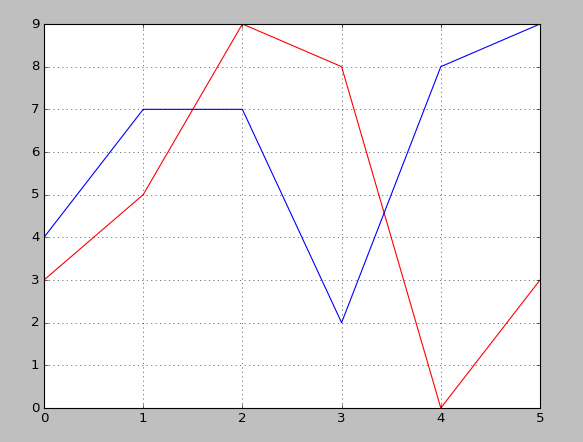
\includegraphics[scale=0.5]{../listes/ecran-liste-cours-visualisation}
\end{center}

\begin{lstlisting}
import matplotlib.pyplot as plt

liste1 = [3,5,9,8,0,3]
liste2 = [4,7,7,2,8,9]

plt.plot(liste1,color="red")
plt.plot(liste2,color="blue")
plt.grid()
plt.show()
\end{lstlisting}


\textbf{Principales fonctions.}

\begin{itemize}
  \item \ci{plt.plot(liste)} trace les points d'une liste (sous la forme $(i,\ell_i)$) et les joint. 
  \item \ci{plt.plot(listex,listey)} trace les points d'une liste (sous la forme $(x_i,y_i)$ où $x_i$ parcourt la première liste et $y_i$ la seconde).    
  \item \ci{plt.scatter(x,y,color='red',s=100)} affiche un point en $(x,y)$ (d'une grosseur \ci{s}).
  \item \ci{plt.grid()} trace une grille.  
  \item \ci{plt.show()} affiche tout. 
  \item \ci{plt.close()} termine le tracé.
  
  \item \ci{plt.xlim(xmin,xmax)} définit l'intervalle des $x$.
  \item \ci{plt.ylim(ymin,ymax)} définit l'intervalle des $y$.
  \item \ci{plt.axis('equal')} impose un repère orthonormé.  
\end{itemize}

%%%%%%%%%%%%%%%%%%%%%%%%%%%%%%%%%%%%%%%%%%%%%%%%%%%%
\section{Tkinter}


%---------------------------------------------------
\subsection{Graphiques}

Pour afficher ceci :
\begin{center}
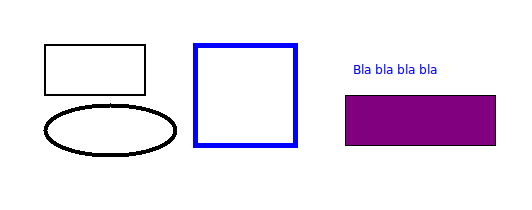
\includegraphics[scale=0.6]{../statistique/ecran-stat-cours-intro}
\end{center}
le code est :
\begin{lstlisting}
# Module tkinter
from tkinter import *

# Fenêtre tkinter
root = Tk()
        
canvas = Canvas(root, width=800, height=600, background="white")
canvas.pack(fill="both", expand=True)

# Un rectangle
canvas.create_rectangle(50,50,150,100,width=2)

# Un rectangle à gros bords bleus
canvas.create_rectangle(200,50,300,150,width=5,outline="blue")

# Un rectangle rempli de violet
canvas.create_rectangle(350,100,500,150,fill="purple")

# Un ovale
canvas.create_oval(50,110,180,160,width=4)

# Du texte
canvas.create_text(400,75,text="Bla bla bla bla",fill="blue")

# Ouverture de la fenêtre
root.mainloop()
\end{lstlisting}


Quelques explications :
\begin{itemize}
  \item Le module \ci{tkinter} nous permet de définir des variables \ci{root} et \ci{canvas} qui définissent une fenêtre graphique (ici de largeur $800$ et de hauteur $600$ pixels).
  On décrit ensuite tout ce que l'on veut ajouter dans la fenêtre. Et enfin, la fenêtre est affichée par la commande \ci{root.mainloop()} (tout à la fin). 
  
    
  \item Attention ! Le repère graphique de la fenêtre a son axe des ordonnées dirigé vers le bas. L'origine $(0,0)$ est le coin en haut à gauche (voir la figure ci-dessous). 
  
  \item Commande pour tracer un rectangle : \ci{create_rectangle(x1,y1,x2,y2)} ; il suffit de préciser les coordonnées $(x_1,y_1)$ et $(x_2,y_2)$ de deux sommets opposés. L'option \ci{width} ajuste l'épaisseur du trait, \ci{outline} définit la couleur de ce trait et \ci{fill} définit la couleur de remplissage.
  
  \item Une ellipse est tracée par la commande \ci{create_oval(x1,y1,x2,y2)}, où $(x_1,y_1)$, $(x_2,y_2)$ sont les coordonnées de deux sommets opposés d'un rectangle encadrant l'ellipse voulue (voir la figure). On obtient un cercle lorsque le rectangle correspondant est un carré.  
  
  \item Le texte est affiché par la commande \ci{canvas.create_text()} en précisant les coordonnées $(x,y)$ du point à partir duquel on souhaite afficher le texte. 
  
\end{itemize}

\myfigure{0.8}{
\tikzinput{../statistique/fig-stat-cours-intro}
}

\textbf{Portion de cercle.}
La fonction \ci{create_arc()} n'est pas très intuitive. Il faut penser que l'on dessine un cercle, en précisant les coordonnées de deux sommets opposés d'un carré qui l'entoure, puis en précisant l'angle de début et l'angle du secteur (en degrés). 

\centerline{\ci{canvas.create_arc(x1,y1,x2,y2,start=debut_angle,extent=mon_angle)}}


\myfigure{0.8}{
\tikzinput{../statistique/fig-stat-arc}
}
L'option \ci{style=PIESLICE} affiche un secteur au lieu d'un arc. 


%---------------------------------------------------
\subsection{Boutons}

Il est plus ergonomique d'afficher des fenêtres dans lesquelles les actions sont exécutées en cliquant sur des boutons.

Voici un petit programme qui affiche une fenêtre avec deux boutons. Le premier bouton change la couleur du rectangle, le second termine le programme.
\begin{center}
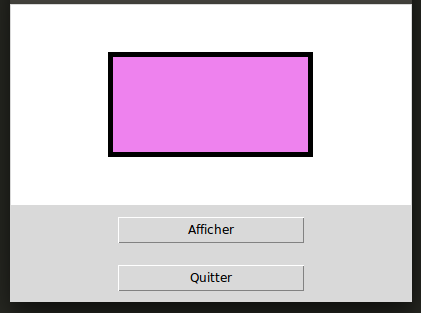
\includegraphics[scale=0.6]{../statistique/ecran-stat-cours-boutons}
\end{center}
Le code est :
\begin{lstlisting}
from tkinter import *
from random import *

root = Tk()     
canvas = Canvas(root, width=400, height=200, background="white")
canvas.pack(fill="both", expand=True)

def action_bouton():
    canvas.delete("all")         # Efface tout
    couleurs = ["red","orange","yellow","green","cyan","blue","violet","purple"]
    coul = choice(couleurs)      # Couleur au hasard
    canvas.create_rectangle(100,50,300,150,width=5,fill=coul)
    return

bouton_couleur = Button(root,text="Afficher", width=20, command=action_bouton)
bouton_couleur.pack()

bouton_quitter = Button(root,text="Quitter", width=20, command=root.quit)
bouton_quitter.pack()

root.mainloop()
\end{lstlisting}

Quelques explications :
\begin{itemize}
  \item On crée un bouton par la commande \ci{Button}. L'option \ci{text} personnalise le texte qui s'affiche sur le bouton. On ajoute le bouton créé à la fenêtre par la méthode \ci{pack}.
  \item Le plus important est l'action associée au bouton ! C'est l'option \ci{command} qui reçoit le nom de la fonction à exécuter lorsque le bouton est cliqué. Pour notre exemple \ci{command=action_bouton} associe au clic sur le bouton un changement de couleur.
  
  \item Attention ! il faut donner le nom de la fonction sans parenthèses : \ci{commande=ma_fonction} et pas \ci{command=ma_fonction()}.
  
  \item Pour associer au bouton \og{}Quitter\fg{} la fermeture du programme, l'argument est \ci{command=root.quit}.
  
  \item La commande \ci{canvas.delete("all")} efface tous les dessins de notre fenêtre graphique.
  
\end{itemize}

%---------------------------------------------------
\subsection{Texte}

Voici comment afficher du texte avec \Python{} et le module des fenêtres graphiques \ci{tkinter}.

\begin{center}

\includegraphics[scale=0.6]{../markdown/ecran-markdown-7}
\end{center}
Le code est :
\begin{lstlisting}
from tkinter import *
from tkinter.font import Font
# Fenêtre tkinter
root = Tk() 
canvas = Canvas(root, width=800, height=600, background="white")
canvas.pack(fill="both", expand=True)
# Fonte
mafonte = Font(family="Times", size=20)
# Le texte
canvas.create_text(100,100, text="Du texte avec Python !", 
anchor=NW, font=mafonte, fill="blue")
# Ouverture de la fenêtre
root.mainloop()
\end{lstlisting}



Quelques explications :
\begin{itemize}
%  \item \ci{root}, \ci{canvas} sont les variables qui définissent une fenêtre graphique (ici de largeur $800$ et de hauteur $600$ pixels). Cette fenêtre est visualisée par la commande de la fin : \ci{root.mainloop()}.
%  
%  \item On rappelle que pour le repère graphique l'axe des ordonnées est dirigé vers le bas. Pour définir un rectangle, il suffit de préciser les coordonnées 
%  $(x_1,y_1)$, $(x_2,y_2)$ de deux sommets opposés (voir la figure ci-dessous). 
  
  \item Le texte est affiché par la fonction \ci{canvas.create_text()}. Il faut préciser les coordonnées $(x,y)$ du point à partir duquel l'on souhaite afficher le texte. 
  
  \item L'option \ci{text} permet de passer la chaîne de caractères à afficher.
  
  \item L'option \ci{anchor} permet de préciser le point d'ancrage du texte, \ci{anchor=NW} signifie que la zone de texte est ancrée au point Nord-Ouest (NW) (voir la figure ci-dessous).
  
  \item L'option \ci{fill} permet de préciser la couleur du texte.
  
  \item L'option \ci{font} permet de définir la fonte (c'est-à-dire le style et la taille des caractères). Voici des exemples de fontes, à toi de les tester :
  \begin{itemize}
    \item \ci{Font(family="Times", size=20)} 
    \item \ci{Font(family="Courier", size=16, weight="bold")} en \textbf{gras}
    \item \ci{Font(family="Helvetica", size=16, slant="italic")} en \emph{italique}
  \end{itemize}  
\end{itemize}

\myfigure{0.7}{
\tikzinput{ecran-markdown-8}
}


%---------------------------------------------------
\subsection{Clic de souris}

Voici un petit programme qui affiche une fenêtre graphique. Chaque fois que l'utilisateur clique (avec le bouton gauche de la souris) le programme affiche un petit carré (sur la fenêtre) et affiche \og{}Clic à $x=\ldots$, $y=\ldots$\fg{} (sur la console). 

\begin{lstlisting}
from tkinter import *

# Fenêtre
root = Tk()
canvas = Canvas(root, width=800, height=600, background="white")
canvas.pack(side=LEFT, padx=5, pady=5)

# Capture des clics de souris
def action_clic_souris(event):
    canvas.focus_set()
    x = event.x
    y = event.y
    canvas.create_rectangle(x,y,x+10,y+10,fill="red")
    print("Clic a x =",x,", y =",y)
    return

# Association clic/action
canvas.bind("<Button-1>", action_clic_souris)

# Lancement
root.mainloop()
\end{lstlisting}


Voici quelques explications :
\begin{itemize}
  \item La création de la fenêtre est habituelle. Le programme se termine par le lancement de la fenêtre avec la commande \ci{mainloop()}.
  
  \item Le premier point clé est d'associer un clic de souris à une action, c'est ce que fait la ligne \\
\centerline{\ci{canvas.bind("<Button-1>", action_clic_souris)}}
Chaque fois que le bouton gauche de la souris est cliqué, \Python{} exécute la fonction \ci{action_clic_souris}. Note qu'il n'y a pas de parenthèses pour l'appel à la fonction.

   \item Second point clé : la fonction \ci{action_clic_souris} récupère les coordonnées du clic et ici ensuite fait deux choses : elle affiche un petit rectangle à l'endroit du clic et affiche dans la fenêtre du terminal les coordonnées $(x,y)$.
   
   \item Les coordonnées $x$ et $y$ sont exprimées en pixels ; $(0,0)$ désigne le coin en haut à gauche de la fenêtre (la zone délimitée par \ci{canvas}).
\end{itemize}

%---------------------------------------------------
\subsection{Mouvement}

Voici un programme qui fait se déplacer un petit carré en le faisant rebondir sur les bords de la fenêtre.

\begin{center}
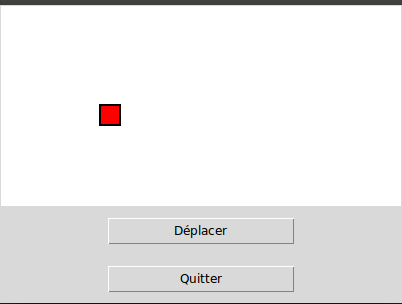
\includegraphics[scale=0.5]{../aleatoire/ecran-alea-cours-mouv}
\end{center}

Voici les points principaux :
\begin{itemize}
  \item Un objet \ci{rect} est défini, c'est une variable globale, de même que ses coordonnées \ci{x0}, \ci{y0}.
  
  \item Cet objet est (un petit peu) déplacé par la fonction \ci{deplacer()} qui décale le rectangle de \ci{(dx,dy)}.
  
  \item Le point clé est que cette fonction sera exécutée une nouvelle fois après un court laps de temps. La commande :\\
  \centerline{\ci{canvas.after(50,deplacer)}}
  demande une nouvelle exécution de la fonction \ci{deplacer()} après un court délai (ici $50$ millisecondes).

  \item La répétition de petits déplacements simule le mouvement.
\end{itemize}

\begin{lstlisting}
from tkinter import *

Largeur = 400
Hauteur = 200

root = Tk()     
canvas = Canvas(root, width=Largeur, height=Hauteur, background="white")
canvas.pack(fill="both", expand=True)

# Les coordonnées et la vitesse
x0, y0 = 100,100
dx = +5  # Vitesse horizontale
dy = +2  # Vitesse verticale

# Le rectangle à déplacer
rect = canvas.create_rectangle(x0,y0,x0+20,y0+20,width=2,fill="red")

# Fonction principale
def deplacer():
    global x0, y0, dx, dy

    x0 = x0 + dx  # Nouvelle abscisse
    y0 = y0 + dy  # Nouvelle ordonnée

    canvas.coords(rect,x0,y0,x0+20,y0+20)  # Déplacement

    if x0 < 0 or x0 > Largeur:
        dx = -dx  # Changement de sens horizontal
    if y0 < 0 or y0 > Hauteur:
        dy = -dy  # Changement de sens vertical

    canvas.after(50,deplacer)  # Appel après 50 millisecondes
 
    return
    
# Fonction pour le bouton
def action_deplacer():
    deplacer()
    return

# Boutons
bouton_couleur = Button(root,text="Déplacer", width=20, command=action_deplacer)
bouton_couleur.pack(pady=10)

bouton_quitter = Button(root,text="Quitter", width=20, command=root.quit)
bouton_quitter.pack(side=BOTTOM, pady=10)

root.mainloop()
\end{lstlisting}



\end{document}
